\documentclass[11pt,a4paper]{article}
\usepackage[spanish,es-nodecimaldot]{babel}	% Utilizar español
\usepackage[utf8]{inputenc}					% Caracteres UTF-8
\usepackage{graphicx}						% Imagenes
\usepackage[hidelinks]{hyperref}			% Poner enlaces sin marcarlos en rojo
\usepackage{fancyhdr}						% Modificar encabezados y pies de pagina
\usepackage{float}							% Insertar figuras
\usepackage[textwidth=390pt]{geometry}		% Anchura de la pagina
\usepackage[nottoc]{tocbibind}				% Referencias (no incluir num pagina indice en Indice)
\usepackage{enumitem}						% Permitir enumerate con distintos simbolos
\usepackage[T1]{fontenc}					% Usar textsc en sections
\usepackage{amsmath}						% Símbolos matemáticos

% Comando para poner el nombre de la asignatura
\newcommand{\asignatura}{Visión por Computador}
\newcommand{\autor}{Vladislav Nikolov Vasilev}
\newcommand{\titulo}{Trabajo 1}
\newcommand{\subtitulo}{Cuestiones de teoría}
\newcommand{\answer}{\noindent\textbf{Solución}}
\newcommand{\question}[1]{\noindent\textbf{#1}}
\newcommand{\nonumbersection}[1]{\section*{#1}\addcontentsline{toc}{section}{#1}}

% Configuracion de encabezados y pies de pagina
\pagestyle{fancy}
\lhead{\autor{}}
\rhead{\asignatura{}}
\lfoot{Grado en Ingeniería Informática}
\cfoot{}
\rfoot{\thepage}
\renewcommand{\headrulewidth}{0.4pt}		% Linea cabeza de pagina
\renewcommand{\footrulewidth}{0.4pt}		% Linea pie de pagina

\begin{document}
\pagenumbering{gobble}

% Pagina de titulo
\begin{titlepage}

\begin{minipage}{\textwidth}

\centering

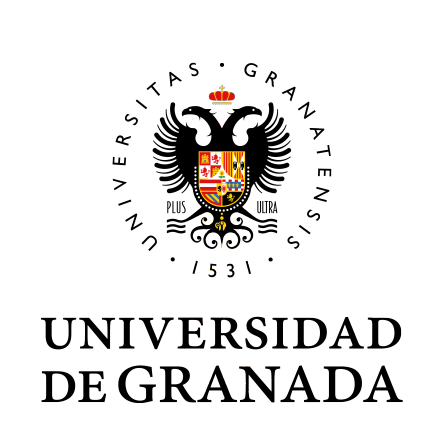
\includegraphics[scale=0.5]{img/ugr.png}\\

\textsc{\Large \asignatura{}\\[0.2cm]}
\textsc{GRADO EN INGENIERÍA INFORMÁTICA}\\[1cm]

\noindent\rule[-1ex]{\textwidth}{1pt}\\[1.5ex]
\textsc{{\Huge \titulo\\[0.5ex]}}
\textsc{{\Large \subtitulo\\}}
\noindent\rule[-1ex]{\textwidth}{2pt}\\[3.5ex]

\end{minipage}

\vspace{0.5cm}

\begin{minipage}{\textwidth}

\centering

\textbf{Autor}\\ {\autor{}}\\[2.5ex]
\textbf{Rama}\\ {Computación y Sistemas Inteligentes}\\[2.5ex]
\vspace{0.3cm}


\includegraphics[scale=0.3]{img/etsiit.jpeg}

\vspace{0.7cm}
\textsc{Escuela Técnica Superior de Ingenierías Informática y de Telecomunicación}\\
\vspace{1cm}
\textsc{Curso 2018-2019}
\end{minipage}
\end{titlepage}

\pagenumbering{arabic}
\tableofcontents
\thispagestyle{empty}				% No usar estilo en la pagina de indice

\newpage

\setlength{\parskip}{1em}

\nonumbersection{Ejercicio 1}

\question{Diga en una sola frase cuál cree que es el objetivo principal de la Visión por Computador. Diga también cuál es la
principal propiedad de las imágenes de cara a la creación de algoritmos que la procesen.}

\answer

El objetivo principal de la Visión por Computador es el procesamiento de imágenes reales o sintéticas, en movimiento
o no, mediante técnicas matemáticas y algorítmicas con el fin de poder entenderlas, valiéndose para ello de la información
semátnica y/o geométrica que puede ser extraída de dichas imágenes.

La principal propiedad de las imágenes de cara a la creación de algoritmos que la procesen es la existencia de una dependencia
entre un píxel y los píxels vecinos de éste, lo cuál implica que los vecinos de un píxel tienen un valor similar a éste. Esta
dependencia es solo local, no global; no se puede asegurar de forma cierta que exista una dependencia entre los píxels de una
región concreta y los de otra muy distante.

\nonumbersection{Ejercicio 2}

\question{Expresar las diferencias y semejanzas entre las operaciones de correlación y convolución. Dar una interpretación de
cada una de ellas que en el contexto de uso en visión por computador.}

\answer

Tanto la correlación como la convolución son operaciones que sirven para aplicar filtros lineales, los cuáles realizan
una combinación lineal de un píxel en concreto y de sus vecinos para obtener uno nuevo. Esto también implica que la salida
depende de los vecinos del píxel, y no de cómo éstos estén distribuidos. Ambas operaciones coinciden cuando la máscara
a aplicar es simétrica en ambos ejes. Además, la forma de aplicarla es la misma, ya que se va recorriendo la imágen píxel
por píxel y se aplica la operación.

Al ser ambas operaciones lineales, cumplen la propiedad de superposición, es decir, que permiten descomponer un problema
lineal complejo en uno más sencillo. Esto se puede ver de la siguiente forma:

\begin{equation}
\label{eq:superposition}
h * (f_1 + f_2) = (h * f_1) + (h * f_2)
\end{equation}

Y, además de eso, ambas operaciones son \textit{shift-invariant}, lo cuál viene a significar que la salida no depende de la
posición del vecindario, si no del vecindario como tal. Es decir, podríamos desplazar la imágen, pero el resultado sería
el mismo, solo que desplazado, en función del desplazamiento que hayamos hecho.

Sin embargo, ambas operaciones presentan algunas diferencias. La más importante de ellas es que la convolución realiza
un giro de la máscara, rotándola en cada uno de los dos ejes antes de aplicarla. Como resultado de esto, las fórmulas
de las dos operaciones son diferentes:

\begin{itemize}
	\item Para la fórmula de la correlación, la cuál se expresa como $G = H \otimes F$, siendo $F$ la imágen de entrada,
	$H$ el filtro y $G$ la imágen de salida, tenemos la siguiente expresión:
	
	\begin{equation}
		G[i, j] = \sum_{u=-k}^{k}\sum_{v=-k}^{k}H[u,v]F[i+u, j+v]
	\end{equation}
	
	\item Para la fórmula de la convolución, la cuál se expresa como $G = H \star F$, siendo $F$ la imágen de entrada,
	$H$ el filtro y $G$ la imágen de salida, tenemos la siguiente expresión:
	\begin{equation}
		G[i, j] = \sum_{u=-k}^{k}\sum_{v=-k}^{k}H[u,v]F[i-u, j-v]
	\end{equation}
\end{itemize}

Otra diferencia importante es que, al aplicar la máscara de una forma diferente, la convolución tiene algunas propiedades
extra. Algunas de ellas son, por ejemplo, la conmutatividad, la asociatividad, la identidad, entre otras.

Dentro de la visión por computador, la correlación se suele utilizar para el \textit{template matching} o búsqueda de patrones
dentro de una imágen, buscando la posición en la que se podría encontrar el patrón dentro de la imágen. La convolución,
debido a los propiedades mencionadas anteriormente, especialmente por la asociativa, es especialmente
utilizada en la aplicación de filtros que transforman la imágen, ya sean filtros de alisamiento como para detectar bordes.
Esto se debe a que permite componer filtros complejos a partir de más sencillos y aplicarlos posteriormente sobre la imágen,
en vez de ir aplicándolos uno por uno.

\nonumbersection{Ejercicio 3}

\question{¿Cuál es la diferencia ``esencial'' entre el filtro de convolución y el de mediana? Justificar la respuesta.}

\answer

La diferencia principal es que el filtro de convolución es lineal y el de mediana es no lineal. Esto significa que el filtro
de convolución utiliza una combinación lineal de los vecinos de un píxel y el píxel mismo para producir un píxel de salida.
En cambio, el filtro de mediana no hace ningún tipo de combinación lineal de los vecinos, si no que, tal y como indica su
nombre, escoge el valor mediano.

Para ver que la mediana es un filtro no lineal, vamos a probar que no cumple la propiedad de superposición (una de las propiedades
de los filtros lineales), la cuál puede ser vista en \eqref{eq:superposition}.

Para ello, vamos a suponer que tenemos dos vectores del mismo tamaño, a los cuáles llamaremos $v_1$ y $v_2$. Tenemos que
$v_1 = [3, 7, 5, 9, 4]$ y $v_2 = [2, 6, 8, 1, 3]$. Vamos a calcular cuál es la mediana de cada vector, primero por
separado y luego para la suma de los dos vectores, y veremos si coincide o no. En caso de coincidir, se cumpliría la
propiedad de superposición, y por tanto, el filtro sería lineal. En caso contrario, no se cumpliría, y no lo sería.

Tenemos que la mediana para cada vector es la siguiente:

\[mediana(v_1) = 5 \]
\[mediana(v_2) = 3 \]

Si sumamos los resultados, obtenemos:

\[mediana(v_1) + mediana(v_2) = 8\]

Ahora, vamos a ver qué resultado obtenemos para la suma de los dos vectores. Este vector tiene el siguiente valor:

\[v_1 + v_2 = [3, 7, 5, 9, 4] + [2, 6, 8, 1, 3] = [5, 13, 13, 10, 7]\]

Si obtenemos la mediana del vector resultado, obtenemos que es la siguiente:

\[mediana(v_1 + v_2) = 10\]

Y por tanto, tenemos que:

\[mediana(v_1) + mediana(v_2) \neq mediana(v_1 + v_2)\]

Por tanto, hemos probado que el filtro de mediana es no lineal, y por tanto, tiene un comportamiento diferente a la
convolución.

\nonumbersection{Ejercicio 4}

\question{Identifique el ``mecanismo concreto'' que usa un filtro de máscara para transformar una imagen.}

\answer

\nonumbersection{Ejercicio 5}

\question{¿De qué depende que una máscara de convolución pueda ser implementada por convoluciones 1D? Justificar la respuesta.}

\answer

\nonumbersection{Ejercicio 6}

\question{Identificar las diferencias y consecuencias desde el punto de vista teórico y de la implementación entre:
\begin{enumerate}[label=\alph*)]
	\item Primero alisar la imagen y después calcular las derivadas sobre la
imagen alisada.
	\item Primero calcular las imágenes derivadas y después alisar dichas
imágenes.
\end{enumerate}
Justificar los argumentos.
}

\answer

\nonumbersection{Ejercicio 7}

\question{Identifique las funciones de las que podemos extraer pesos correctos
para implementar de forma eficiente la primera derivada de una imagen.
Suponer alisamiento Gaussiano.}

\answer

\nonumbersection{Ejercicio 8}

\question{Identifique las funciones de las que podemos extraer pesos correctos
para implementar de forma eficiente la Laplaciana de una imagen. Suponer
alisamiento Gaussiano.}

\answer

\nonumbersection{Ejercicio 9}

\question{Suponga que le piden implementar de forma eficiente un algoritmo para
el cálculo de la derivada de primer orden sobre una imagen usando
alisamiento Gaussiano. Enumere y explique los pasos necesarios para
llevarlo a cabo.}

\answer

\nonumbersection{Ejercicio 10}

\question{Identifique semejanzas y diferencias entre la pirámide gaussiana y
el espacio de escalas de una imagen, ¿cuándo usar una u otra? Justificar
los argumentos.}

\answer

\nonumbersection{Ejercicio 11}

\question{¿Bajo qué condiciones podemos garantizar una perfecta reconstrucción
de una imagen a partir de su pirámide Laplaciana? Dar argumentos y
discutir las opciones que considere necesario.}

\answer

\nonumbersection{Ejercicio 12}

\question{ ¿Cuáles son las contribuciones más relevantes del algoritmo de
Canny al cálculo de los contornos sobre una imagen? ¿Existe alguna
conexión entre las máscaras de Sobel y el algoritmo de Canny? Justificar
la respuesta.}

\answer

\nonumbersection{Ejercicio 13}

\question{- Identificar pros y contras de k-medias como mecanismo para crear un
vocabulario visual a partir del cual poder caracterizar patrones. ¿Qué
ganamos y que perdemos? Justificar los argumentos.}

\answer

\nonumbersection{Ejercicio 14}

\question{Identifique pros y contras del modelo de “Bolsa de Palabras” como
mecanismo para caracterizar el contenido de una imagen. ¿Qué ganamos y
que perdemos? Justificar los argumentos.}

\answer

\nonumbersection{Ejercicio 15}

\question{Suponga que dispone de un conjunto de imágenes de dos tipos de
clases bien diferenciadas. Suponga que conoce como implementar de forma
eficiente el cálculo de las derivadas hasta el orden N de la imagen.
Describa como crear un algoritmo que permita diferenciar, con garantías,
imágenes de ambas clases. Justificar cada uno de los pasos que proponga.}

\answer

\newpage

\begin{thebibliography}{5}

\bibitem{nombre-referencia}
Texto referencia
\\\url{https://url.referencia.com}

\end{thebibliography}

\end{document}

